\begin{frame}
  \begin{center}
    \Huge Problem definition
  \end{center}
\end{frame}

\begin{frame}
  \frametitle{Problem definition}
  Let
  \begin{itemize}
    \item \blue{$D(V = \{s\} \cup V^{+} \cup \{t\}, A)$} be the digraph, where
    \begin{itemize}
      \item \blue{$s$} is the source node; and 
      \item \blue{$t$} is the target node.
    \end{itemize}
    \item \blue{$c_a \in \mathbb{R}$} be the arc \blue{$a \in A$} cost;
    \item \blue{$R$} be the set of resources;
    \item \blue{$d^r_a \in \mathbb{R}$} be the metric resource \blue{$r \in R$} consumption of the arc \blue{$a \in A$};
    \item \blue{$w^r_i = [b^r_i, e^r_i]$} be the resource \blue{$r \in R$} window of the node \blue{$i \in V$}.
  \end{itemize}
\end{frame}

\begin{frame}
  \frametitle{Problem definition}
  Let
  \begin{itemize}
    \item \blue{$P$} be an elementary resource constrained \blue{$s$}-\blue{$t$}-path in \blue{$D$}; and
    \item \blue{$S_i^r$} be the resource \blue{$r \in R$} consumption of node \blue{$i \in V(P)$},
  such that \blue{$\forall (i, j) \in A(P) (\forall r \in R (S_j^r = \text{max} \{S_i^r + d_{ij}^r, b_j^r\} \leqslant e_j^r))$}.
  \end{itemize}
  The ERCSPP consists in finding the shortest elementary resource constrained \blue{$s$}-\blue{$t$}-path \blue{$P$} in \blue{$D$}.
\end{frame}

\begin{frame}
  \frametitle{Problem definition}
  \blue{$c_a: (d^1_a, d^2_a)$}
  \begin{figure}[H]
    \centering
    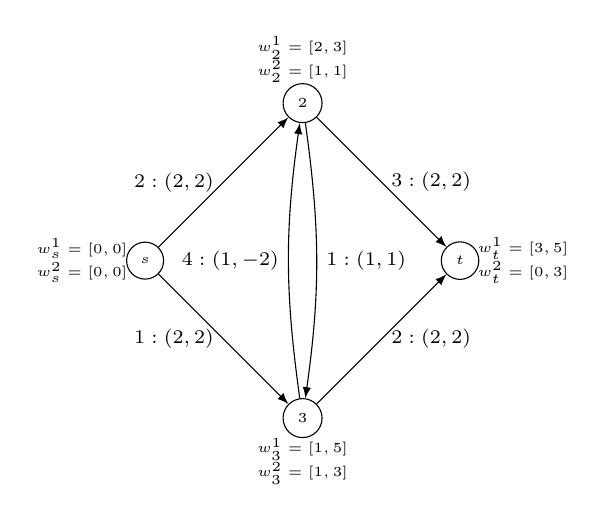
\begin{tikzpicture}[font=\tiny]
      %nodes
      \node at (-0.8, 0.15) {\blue{$w_s^1 = [0,0]$}};
      \node at (-0.8, -0.15) {\blue{$w_s^2 = [0,0]$}};
      \node[circle, draw] (s) at (0, 0) {\blue{$s$}};
      \node at (2, 2.7) {\blue{$w_2^1 = [2, 3]$}};
      \node at (2, 2.4) {\blue{$w_2^2 = [1, 1]$}};
      \node[circle, draw] (a) at (2, 2) {\blue{$2$}};
      \node at (2, -2.4) {\blue{$w_3^1 = [1, 5]$}};
      \node at (2, -2.7) {\blue{$w_3^2 = [1, 3]$}};
      \node[circle, draw] (b) at (2, -2) {\blue{$3$}};
      \node at (4.8, 0.15) {\blue{$w_t^1 = [3, 5]$}};
      \node at (4.8, -0.15) {\blue{$w_t^2 = [0, 3]$}};
      \node[circle, draw] (t) at (4, 0) {\blue{$t$}};
      %edges
      \path [draw,-latex] (s) to node[left]{\scriptsize\blue{$2: (2, 2)$}} (a);
      \path [draw,-latex] (s) to node[left]{\scriptsize\blue{$1: (2, 2)$}} (b);
      \path [draw,-latex] (a) to node[right]{\scriptsize\blue{$3: (2, 2)$}} (t);
      \path [draw,-latex] (b) to node[right]{\scriptsize\blue{$2: (2, 2)$}} (t);
      \path [draw,-latex] (a) edge [bend left=8] node[right]{\scriptsize\blue{$1: (1, 1)$}} (b);
      \path [draw,-latex] (b) edge [bend left=8] node[left]{\scriptsize\blue{$4: (1, -2)$}} (a);
    \end{tikzpicture}
    \caption{A ERCSPP instance digraph example.}
  \end{figure}
\end{frame}

\begin{frame}
  \frametitle{Problem definition}
  \blue{$c_a: (d^1_a, d^2_a)$}
  \begin{figure}[H]
    \centering
    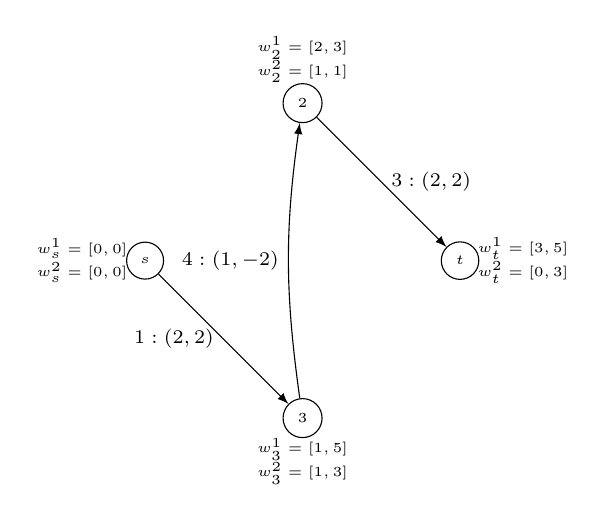
\begin{tikzpicture}[font=\tiny]
      %nodes
      \node at (-0.8, 0.15) {\blue{$w_s^1 = [0,0]$}};
      \node at (-0.8, -0.15) {\blue{$w_s^2 = [0,0]$}};
      \node[circle, draw] (s) at (0, 0) {\blue{$s$}};
      \node at (2, 2.7) {\blue{$w_2^1 = [2, 3]$}};
      \node at (2, 2.4) {\blue{$w_2^2 = [1, 1]$}};
      \node[circle, draw] (a) at (2, 2) {\blue{$2$}};
      \node at (2, -2.4) {\blue{$w_3^1 = [1, 5]$}};
      \node at (2, -2.7) {\blue{$w_3^2 = [1, 3]$}};
      \node[circle, draw] (b) at (2, -2) {\blue{$3$}};
      \node at (4.8, 0.15) {\blue{$w_t^1 = [3, 5]$}};
      \node at (4.8, -0.15) {\blue{$w_t^2 = [0, 3]$}};
      \node[circle, draw] (t) at (4, 0) {\blue{$t$}};
      %edges
      \path [draw,-latex] (s) to node[left]{\scriptsize\blue{$1: (2, 2)$}} (b);
      \path [draw,-latex] (b) edge [bend left=8] node[left]{\scriptsize\blue{$4: (1, -2)$}} (a);
      \path [draw,-latex] (a) to node[right]{\scriptsize\blue{$3: (2, 2)$}} (t);
    \end{tikzpicture}
    \caption{The solution of the previous instance.}
  \end{figure}
\end{frame}
